% !TEX root = main.tex
\section{Introduzione e Modello Analitico}

L'obiettivo di questa relazione è l'analisi in frequenza e la successiva sintesi del segnale periodico $y(t)$ assegnato. Al fine di semplificare il calcolo dei coefficienti dello sviluppo in serie di Fourier, risulta conveniente sfruttare la linearità dell'operatore trasformata e scomporre il segnale in componenti elementari note.

Osservando l'andamento del segnale in un singolo periodo $T_0$, e centrando l'asse dei tempi, è possibile modellare $y(t)$ come la sovrapposizione lineare di $y_1(t)$ (segnale $\Delta$) e $y_2(t)$ (segnale $\Pi$).

Questo è il modo più efficiente di calcolare le caratteristiche del segnale, in quanto le proprietà delle funzioni $\Delta$ e $\Pi$ sono già note.

I parametri calcolati a partire dal numero di lettere del cognome ("D'Amico" $\rightarrow N=6$) sono:
\begin{itemize}
    \item $A = \lceil \frac{N}{2} \rceil = \lceil \frac{6}{2} \rceil = 3 \text{ V}$
    \item $T_0 = \frac{1}{N} \text{ ms} = \frac{1}{6} \text{ ms}$
\end{itemize}

L'espressione analitica nel periodo $t \in \left[-\frac{T_0}{2}, \frac{T_0}{2}\right]$ risulta essere:
\begin{equation}
    y(t) = y_1(t) + y_2(t) = A \cdot \Delta\left(\frac{t}{T_0/2}\right) + \frac{A}{2} \Pi\left(\frac{t}{T_0/2}\right)
\end{equation}

\subsection{Sfruttamento delle Simmetrie}
Una caratteristica importante da notare subito è che sia $\Delta(\cdot)$ che $\Pi(\cdot)$ sono \textbf{funzioni pari}. Di conseguenza, anche la loro somma $y(t)$ è una funzione pari. Questo ci garantisce in anticipo che i coefficienti dello sviluppo in serie di Fourier saranno puramente reali (parte immaginaria nulla).

\subsection{Rappresentazione Grafica delle Componenti}
Di seguito viene illustrata la scomposizione grafica del segnale (con valori normalizzati $A=2, T_0=4$ per chiarezza visiva), mostrando prima le singole componenti e infine il segnale risultante.

\vspace{0.5cm}

\begin{center}
    \begin{minipage}{0.48\textwidth}
        \centering
        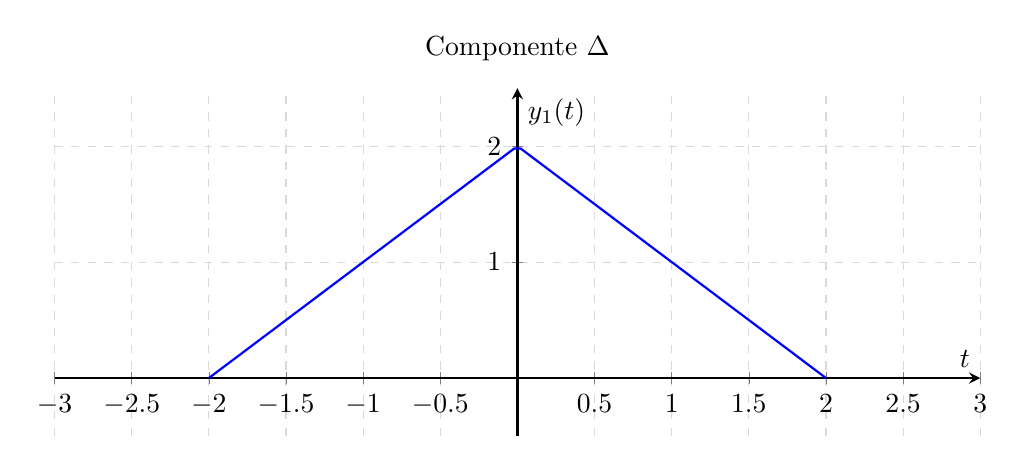
\begin{tikzpicture}
            \begin{axis}[
                    width=1.1\textwidth,
                    height=6cm,
                    axis lines=middle,
                    xmin=-3, xmax=3,
                    ymin=-0.5, ymax=2.5,
                    xlabel={$t$},
                    ylabel={$y_1(t)$},
                    grid=both,
                    grid style={dashed, gray!30},
                    thick,
                    title={Componente $\Delta$}
                ]
                \addplot[
                    domain=-2:2,
                    samples=100,
                    color=blue
                ]
                {2 * max(0, 1 - abs(x)/2)};
            \end{axis}
        \end{tikzpicture}
    \end{minipage}
    \hfill
    \begin{minipage}{0.48\textwidth}
        \centering
        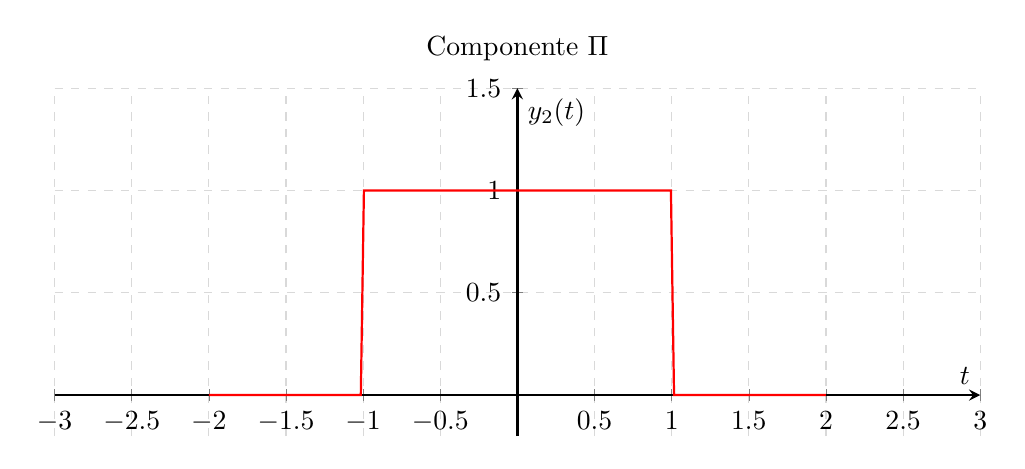
\begin{tikzpicture}
            \begin{axis}[
                    width=1.1\textwidth,
                    height=6cm,
                    axis lines=middle,
                    xmin=-3, xmax=3,
                    ymin=-0.2, ymax=1.5,
                    xlabel={$t$},
                    ylabel={$y_2(t)$},
                    grid=both,
                    grid style={dashed, gray!30},
                    thick,
                    title={Componente $\Pi$}
                ]
                \addplot[
                    domain=-2:2,
                    samples=200,
                    color=red
                ]
                {(abs(x) <= 1) ? 1 : 0};
            \end{axis}
        \end{tikzpicture}
    \end{minipage}
\end{center}

\newpage

\vspace{0.8cm}

\begin{center}
    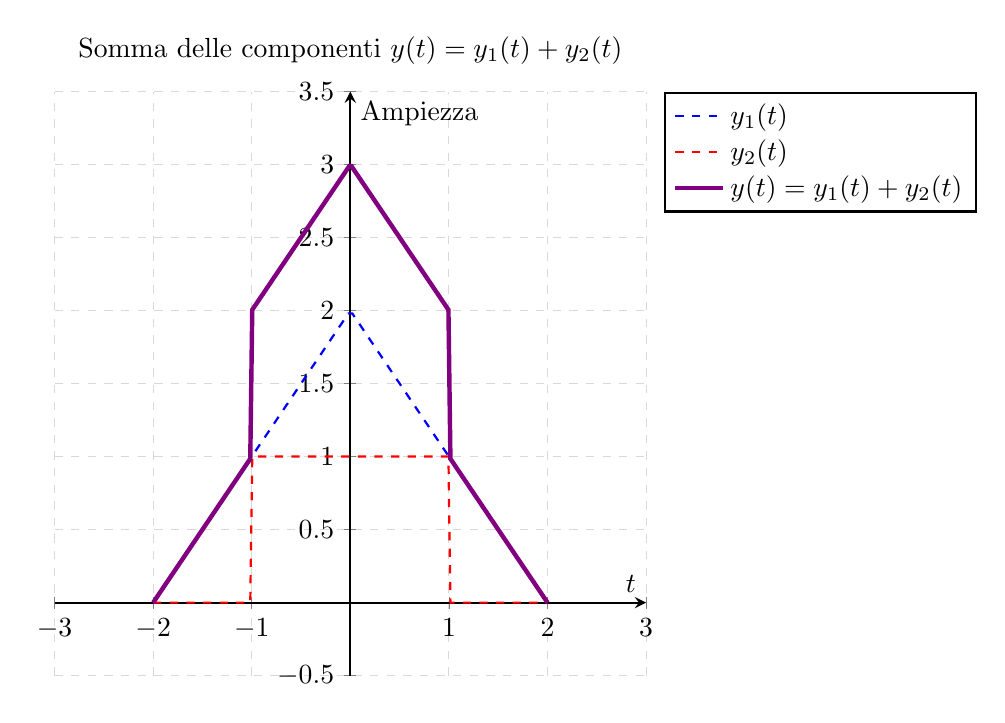
\begin{tikzpicture}
        \begin{axis}[
                width=0.75\textwidth,
                height=9cm,
                axis lines=middle,
                xmin=-3, xmax=3,
                ymin=-0.5, ymax=3.5,
                xlabel={$t$},
                ylabel={Ampiezza},
                legend pos=outer north east,
                legend cell align={left},
                grid=both,
                grid style={dashed, gray!30},
                thick,
                title={Somma delle componenti $y(t) = y_1(t) + y_2(t)$}
            ]

            % Componente 1: \Delta (y1)
            \addplot[
                domain=-2:2,
                samples=100,
                color=blue,
                dashed
            ]
            {2 * max(0, 1 - abs(x)/2)};
            \addlegendentry{$y_1(t)$}

            % Componente 2: \Pi (y2)
            \addplot[
                domain=-2:2,
                samples=200,
                color=red,
                dashed
            ]
            {(abs(x) <= 1) ? 1 : 0};
            \addlegendentry{$y_2(t)$}

            % Segnale Originale (y)
            \addplot[
                domain=-2:2,
                samples=200,
                color=violet,
                ultra thick
            ]
            {(abs(x) <= 1 ? 1 : 0) + 2 * max(0, 1 - abs(x)/2)};
            \addlegendentry{$y(t) = y_1(t) + y_2(t)$}

        \end{axis}
    \end{tikzpicture}
\end{center}

In corrispondenza dell'istante $t = \pm \frac{T_0}{4}$, la caduta verticale del rettangolo e la pendenza del triangolo si sommano creando in quel punto l'esatto salto di ampiezza $\frac{A}{2}$ mostrato nella figura originale della consegna.

\vspace{0.8cm}
\begin{center}
    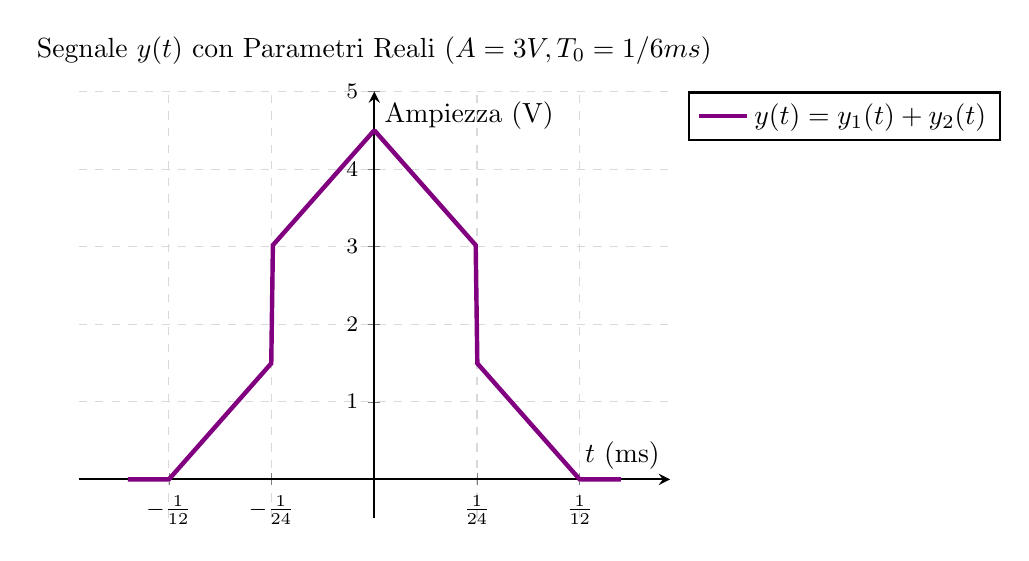
\begin{tikzpicture}
        \begin{axis}[
                width=0.75\textwidth,
                height=7cm,
                axis lines=middle,
                xmin=-0.12, xmax=0.12,
                ymin=-0.5, ymax=5.0,
                xlabel={$t$ (ms)},
                ylabel={Ampiezza (V)},
                xtick={-0.08333, -0.04166, 0, 0.04166, 0.08333},
                xticklabels={$-\frac{1}{12}$, $-\frac{1}{24}$, $0$, $\frac{1}{24}$, $\frac{1}{12}$},
                scaled x ticks=false,
                tick label style={font=\footnotesize},
                grid=both,
                grid style={dashed, gray!30},
                thick,
                legend pos=outer north east,
                legend cell align={left},
                title={Segnale $y(t)$ con Parametri Reali ($A=3\text{ V}, T_0=1/6\text{ ms}$)}
            ]

            % Segnale Originale Somma (y)
            \addplot[
                domain=-0.1:0.1,
                samples=300,
                color=violet,
                ultra thick
            ]
            {(abs(x*24) <= 1 ? 1.5 : 0) + 3 * max(0, 1 - abs(x*12))};
            \addlegendentry{$y(t) = y_1(t) + y_2(t)$}

        \end{axis}
    \end{tikzpicture}
\end{center}

